\state{}{
	 In this problem you will explore the geometry of a sphere $S^2$ of radius $R$.
}

\prob{
	A vector $\vV = \Vtht \vestht + \Vphi \vesphi$ is defined at a point $(\tht, \phi)$ on the sphere.  It is then parallel transported around the circle of constant $\tht$ with $\phi \to \phi + 2\pi$.  What are its resulting components?  What is its length?
}

\sol{
	From Lecture~7, the parallel transport equation is
	\eqn{pt}{
		\dv{\Vb}{\tau} + \Gambsma \Vm(\tau) \pdv{\xa}{\tau} = 0.
	}
	Let $\uv = \dv*{\vx}{\tau}$ be the vector tangent to the curve along which we are transporting $\vV$.
	
	For our problem, let $\vx = (\thto, \phi)$, with $\thto$ constant.  Then $\tau \to \phi$, and so $\uv = (0, 1)$.  Then Eq.~\refeq{pt} becomes two expressions, one for $\bet \to \tht$ and one for $\bet \to \phi$.  We have
	\aln{
		0 &= \dv{\Vtht}{\phi} + \Gam^\tht{}_{\mu \phi} \Vm
		= \dv{\Vtht}{\phi} + \Gam^\tht{}_{\tht \phi} \Vtht + \Gam^\tht{}_{\phi \phi} \Vphi
		= \dv{\Vtht}{\phi} - \sin\thto \cos\thto \Vphi, \label{thing3a1} \\
		%
		0 &= \dv{\Vphi}{\phi} + \Gam^\phi{}_{\mu \phi} \Vm
		= \dv{\Vphi}{\phi} + \Gam^\phi{}_{\tht \phi} \Vtht + \Gam^\phi{}_{\phi \phi} \Vphi
		= \dv{\Vphi}{\phi} + \frac{1}{\tan\thto} \Vtht, \label{thing3a2}
	}
	where we have used our commutation coefficients from \ref{1b}.  This gives us a system of equations that we can use to solve for the components of $\vV$.  We can differentiate one of the equations and feed in the other:
	\al{
		0 &= \dv[2]{\Vtht}{\phi} - \sin\thto \cos\thto \dv{\Vphi}{\phi}
		= \dv[2]{\Vtht}{\phi} + \cos^2\thto \Vtht, \\
		%
		0 &= \dv[2]{\Vphi}{\phi} + \frac{1}{\tan\thto} \dv{\Vtht}{\phi}
		= \dv[2]{\Vphi}{\phi} + \cos^2\thto \Vphi.
	}
	The solutions to these equations are~\cite[p.~207]{Swartz}
	\aln{ \label{thing3a}
		\Vtht &= \Cq \cos(\omg \phi) + \Cw \sin(\omg \phi), &
		\Vphi &= \Dq \cos(\omg \phi) + \Dw \sin(\omg \phi),
	}
	where $\omg = \cos\thto$.  Let the coordinates of our vector at $\phi = 0$ be given by $\vV(0) = (\Vthto, \Vphio)$.  Applying this condition to Eq.~\refeq{thing3a} gives us
	\al{
		\Vthto &= \Cq, &
		\Vphio &= \Dq.
	}
	Involving Eqs.~\refeq{thing3a1} and \refeq{thing3a2} as well gives us
	\al{
		\left. \dv{\Vtht}{\phi} \right|_0 &= \sin\thto \cos\thto \Vphi
		= \sin\thto \cos\thto [ \Vphio \cos(\omg \phi) + \Dw \sin(\omg \phi) ]
		= -\Vthto \omg \sin(\omg \phi) + \Cw \omg \cos(\omg \phi), \\
		%
		\left. \dv{\Vphi}{\phi} \right|_0 &= -\frac{1}{\tan\thto} \Vtht
		= -\frac{1}{\tan\thto} [ \Vthto \cos(\omg \phi) + \Cw \sin(\omg \phi) ]
		= -\Vphio \omg \sin(\omg \phi) + \Dw \omg \cos(\omg \phi),
	}
	and solving these two equations for $\Cw$ and $\Dw$ yields
	\al{
		\Cw &= \Vphio \sin\thto, &
		\Dw &= -\frac{\Vthto}{\sin\thto}.
	}
	So referring once more to Eq.~\refeq{thing3a}, we may finally write the components of $\vV$:
	\ans{\eq{
		\vV = \brac{ \Vthto \cos(\omg \phi) + \Vphio \sin\thto \sin(\omg \phi) } \vestht + \brac{ \Vphio \cos(\omg \phi) - \frac{\Vthto}{\sin\thto} \sin(\omg \phi) } \vesphi
	}}%
	with $\omg = \cos\thto$.
	
	We can find the length $V$ using the dot product:
	\al{
		V^2 &= \vV \cdot \vV \\[1ex]
		&= \sgsab \Va \Vb \\[1ex]
		&= \sg_{\tht \tht} \Vtht \Vtht + \sg_{\phi \phi} \Vphi \Vphi \\[1ex]
		&= R^2 \brac{ \Vthto \cos(\omg \phi) + \Vphio \sin\thto \sin(\omg \phi) }^2 + R^2 \sin^2\thto \brac{ \Vphio \cos(\omg \phi) - \frac{\Vthto}{\sin\thto} \sin(\omg \phi) }^2 \\[2ex]
		&= R^2 \brac{ \Vthto \cos(\omg \phi) + \Vphio \sin\thto \sin(\omg \phi) }^2 + R^2 \brac{ \Vphio \sin\thto \cos(\omg \phi) - \Vthto \sin(\omg \phi) }^2 \\[2ex]
		&= R^2 \left[ {\Vthto}^2 \cos^2(\omg \phi) + 2 \Vthto \Vphio \sin\thto \sin(\omg \phi) \cos(\omg \phi) + {\Vphio}^2 \sin^2\thto \sin^2 (\omg \phi) + {\Vphio}^2 \sin^2\thto \cos^2(\omg \phi) \right. \\
		&\hspace{5em} \phantom{=\ } \left. - 2 \Vphio \Vthto \sin\thto \sin(\omg \phi) \cos(\omg \phi) + {\Vthto}^2 \sin^2(\omg \phi) \right] \\[2ex]
		&= R^2 \brac{ {\Vthto}^2 + {\Vphio}^2 \sin^2(\omg \phi) } \\[2ex]
		&= R^2 {\Vthto}^2 + R^2 \sin^2(\omg \phi) {\Vphio}^2,
	}
	where we have used Eq.~\refeq{metric}.  Thus the length of $\vV$ is
	\eq{
		\ans{ V = \sqrt{ R^2 {\Vthto}^2 + R^2 \sin^2(\omg \phi) {\Vphio}^2 }, }
	}
	which is unchanged as we would expect.
}



\prob{
	Write the geodesic equation in $(\tht, \phi)$ angular coordinates.  Show that the solutions are \emph{great circles}, i.e.~circles on the sphere of largest diameter.
}

\sol{
	From Lecture~7, the geodesic equation is
	\eq{
		\dv{\ua}{\tau} + \umm \unn \Gamasmn = 0.
	}
	We have two equations, one with $\alp \to \tht$ and one with $\alp \to \phi$:
	\aln{
		0 &= \dv{\utht}{\tau} + \umm \unn \Gam^\tht{}_{\mu \nu}
		= \dv{\utht}{\tau} + \uphi \uphi \Gam^\tht{}_{\phi \phi}
		= \dv{\utht}{\tau} - \sin\tht \cos\tht {\uphi}^2, \label{thing3b1} \\
		%
		0 &= \dv{\uphi}{\tau} + \umm \unn \Gam^\phi{}_{\mu \nu}
		= \dv{\uphi}{\tau} + \utht \uphi \Gam^\tht{}_{\tht \phi} + \uphi \utht \Gam^\phi{}_{\phi \tht}
		= \dv{\uphi}{\tau} + 2 \frac{1}{\tan\tht} \utht \uphi. \label{thing3b2}
	}
	In order to solve these equations, we choose the initial conditions
	\al{
		\thto &= \frac{\pi}{2}, &
		\phio &= 0, &
		\uphio &= 1, &
		\uthto &= 0.
	}
	This set of initial conditions is completely general because we can always rotate our coordinate system.  Applying these conditions to Eqs.~\refeq{thing3b1} and \refeq{thing3b2},
	\al{
		\left. \dv{\utht}{\tau} \right|_0 &= \sin(\pi / 2) \cos(\pi / 2) = 0, &
		\left. \dv{\uphi}{\tau} \right|_0 &= 0.
	}
	This means both components of $\uv$ are constant, and we have
	\al{
		\uv &= (0, 1)
		\qimplies &
		\dv{\tht}{\tau} &= 0, &
		\dv{\phi}{\tau} &= 1,
	}
	which implies $\tht = \pi / 2$ is constant and $\phi = \tau$.  So our parameterized curve traces out a circle of radius $R$ at $\tht = \pi / 2$.  This is a great circle because its radius is equal to the radius of $S^2$, and we could rotate our coordinate system to transform this to any other great circle. \qed
}



\prob{
	Consider a disk of radius $\eps$ on the sphere.  Working in the limit of small $\eps$, compute the area of the disk to order $\eps^4$.  Compare your results to $\bbR^2$ with the flat metric.
}

\sol{
	We place the disk at the ``top'' of the sphere so its center is at $\tht = 0$.  The area element for a sphere of radius $R$ is $R^2 \sin\tht \ddtht \ddphi$~\cite{Spherical}.  We need to integrate over the surface of the sphere from $\tht = 0$ to $\tht = \eps / R$:
	\eq{
		\ddA = \int_0^{2\pi} \int_0^{\eps / R} R^2 \sin\tht \ddtht \ddphi
		= R^2 \int_0^{2\pi} \ddphi \int_0^{\eps / R} \sin\tht \ddtht
		= 2\pi R^2 \bigg[ -\cos\tht \bigg]_0^{\eps / R}
		= 2\pi R^2 \brac{ 1 - \cos(\frac{\eps}{R}) }.
	}
	The Maclaurin series expansion for $\cos x$ is~\cite{Maclaurin}
	\eq{
		\cos x \approx 1 - \frac{1}{2} x^2 + \frac{1}{24} x^4,
	}
	so our area is
	\eq{
		\ddA = 2\pi R^2 \brac{ \frac{1}{2} \frac{\eps^2}{R^2} - \frac{1}{24} \frac{\eps^4}{R^4} }
		= \ans{ \pi \eps^2 - \frac{\pi}{12} \frac{\eps^4}{R^2}. }
	}
	In $\bbR^2$ with the flat metric, $\ddA = \pi \eps^2$.  So the area on the sphere is smaller.
}


\clearpage
\prob{
	A spherical triangle is made from three points on the sphere pairwise connected by geodesics.  Let the angles on the triangle be $\alp$, $\bet$, and $\gam$.  By drawing pictures, show that $\alp + \bet + \gam$ can be larger than $\pi$.
}

\sol{
	We can draw a triangle on the sphere where $\alp > 0$ and $\bet = \gam = \pi / 2$, so $\alp + \bet + \gam > \pi$.  This is shown in Fig.~\ref{f3d}.
	
	\begin{figure} \centering
		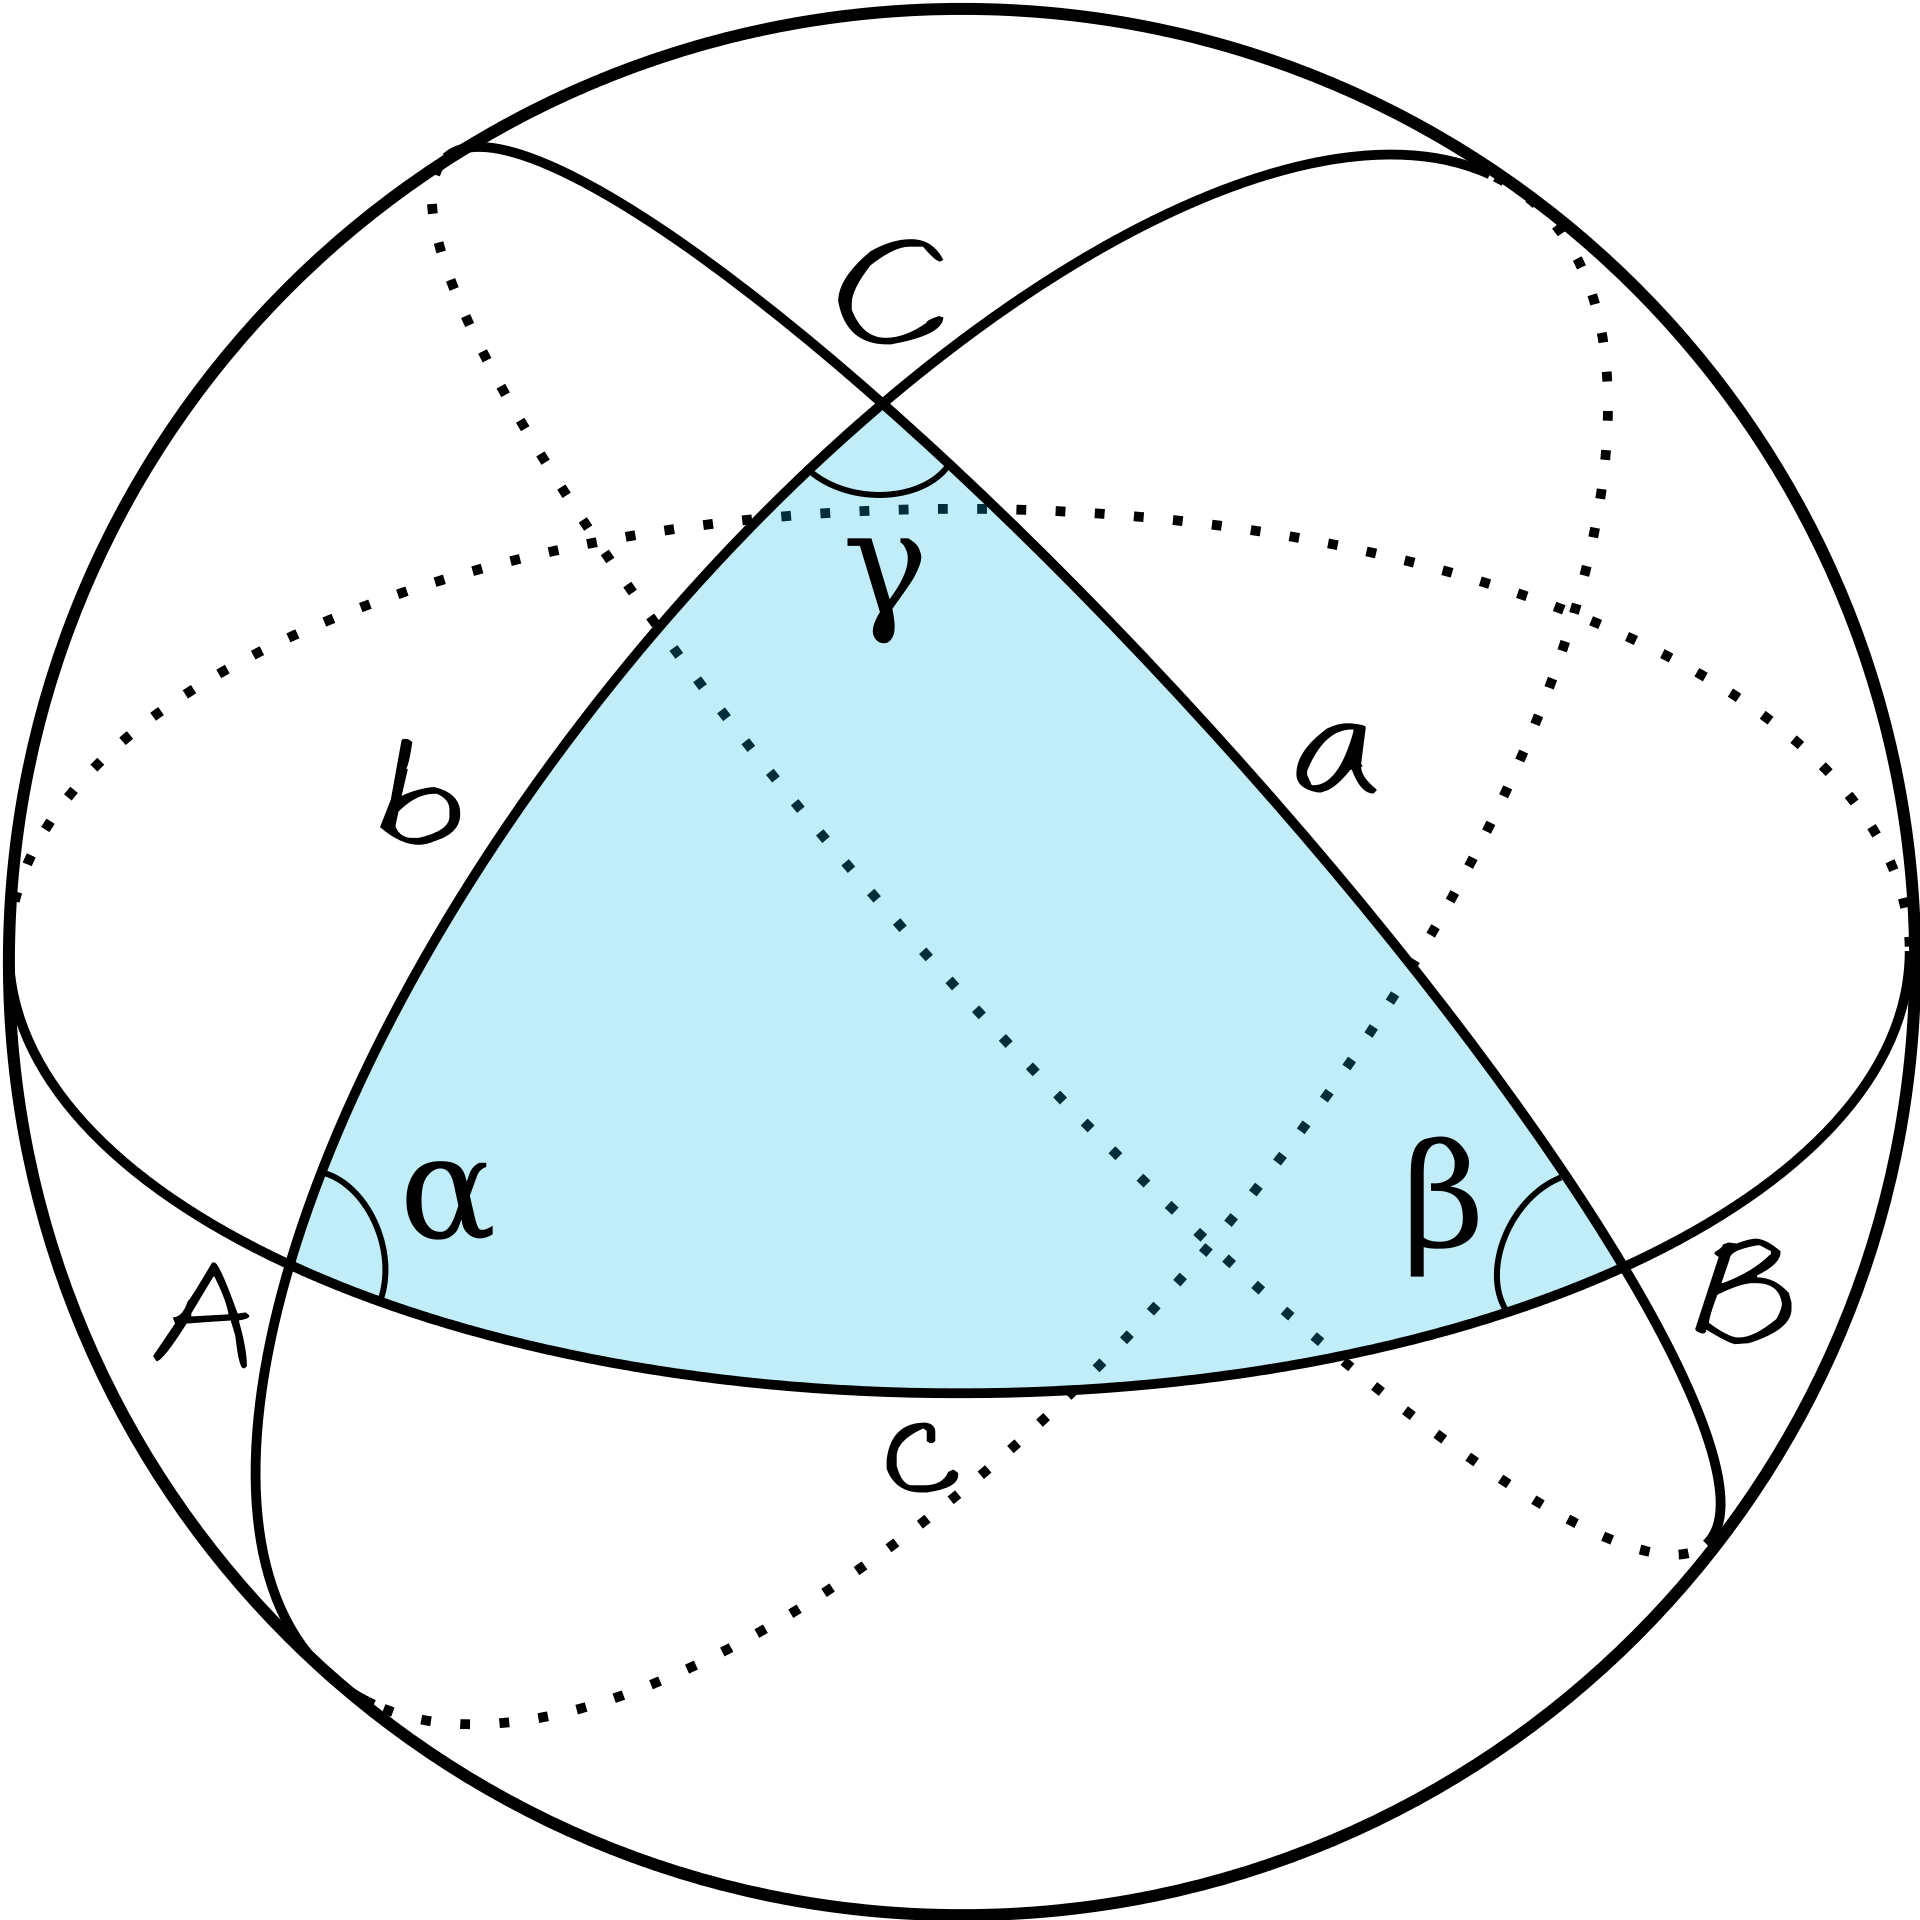
\includegraphics[width=0.3\textwidth]{sphere.png}
		\caption{A triangle on the sphere with $\alp > 0$ and $\bet = \gam = \pi / 2$.}
		\label{f3d}
	\end{figure}
}



\prob{
	Define the excess angle $E$ of a spherical triangle by $E = \alp + \bet + \gam - \pi$.  Prove that the area of the triangle is $R^2 E$.
}

\sol{
	The vertices of any triangle on the great sphere can be defined by the intersection points of three great circles.  In fact, two triangles of identical area are defined this way.  This is illustrated in Fig.~\ref{f3e}(a), with both of the triangles shaded.  Call the area of one of these triangles $\Asabg$.
	
	We can also define a region on the surface of the sphere by the intersection of two great circles at some angle $\tht$.  Two regions identical in area can be defined this way, as illustrated by the shaded areas in Fig.~\ref{f3e}(b)--(d).  Call the area of one of these regions $\Astht$.  We can find its area using
	\eqn{thing3e}{
		\frac{4 \pi R^2}{\pi} = \frac{2 \Astht}{\tht}
		\qimplies
		\Astht = 2 \tht R^2,
	}
	since drawing two great circles separated by angle $\pi$ covers the entire sphere in this manner.
	
	If we add up all of the shaded areas in Fig.~\ref{f3e}(b)--(d), we have covered each of the triangles three times (that is, we have covered $6 \Asabg$) and the rest of the sphere's area once.  The area we have covered can be expressed
	\eq{
		4\pi R^2 + 4 \Asabg = 2 (\Asa + \Asb + \Asg)
		= 4 R^2 (\alp + \bet + \gam),
	}
	using Eq.~\refeq{thing3e}, which implies
	\eq{
		\Asabg = 4 R^2 (\alp + \bet + \gam - \pi)
		= \ans{ 4 R^2 E }
	}
	as we wanted to show. \qed
	
	\begin{figure} \centering
		\begin{tabular}{c c c}
			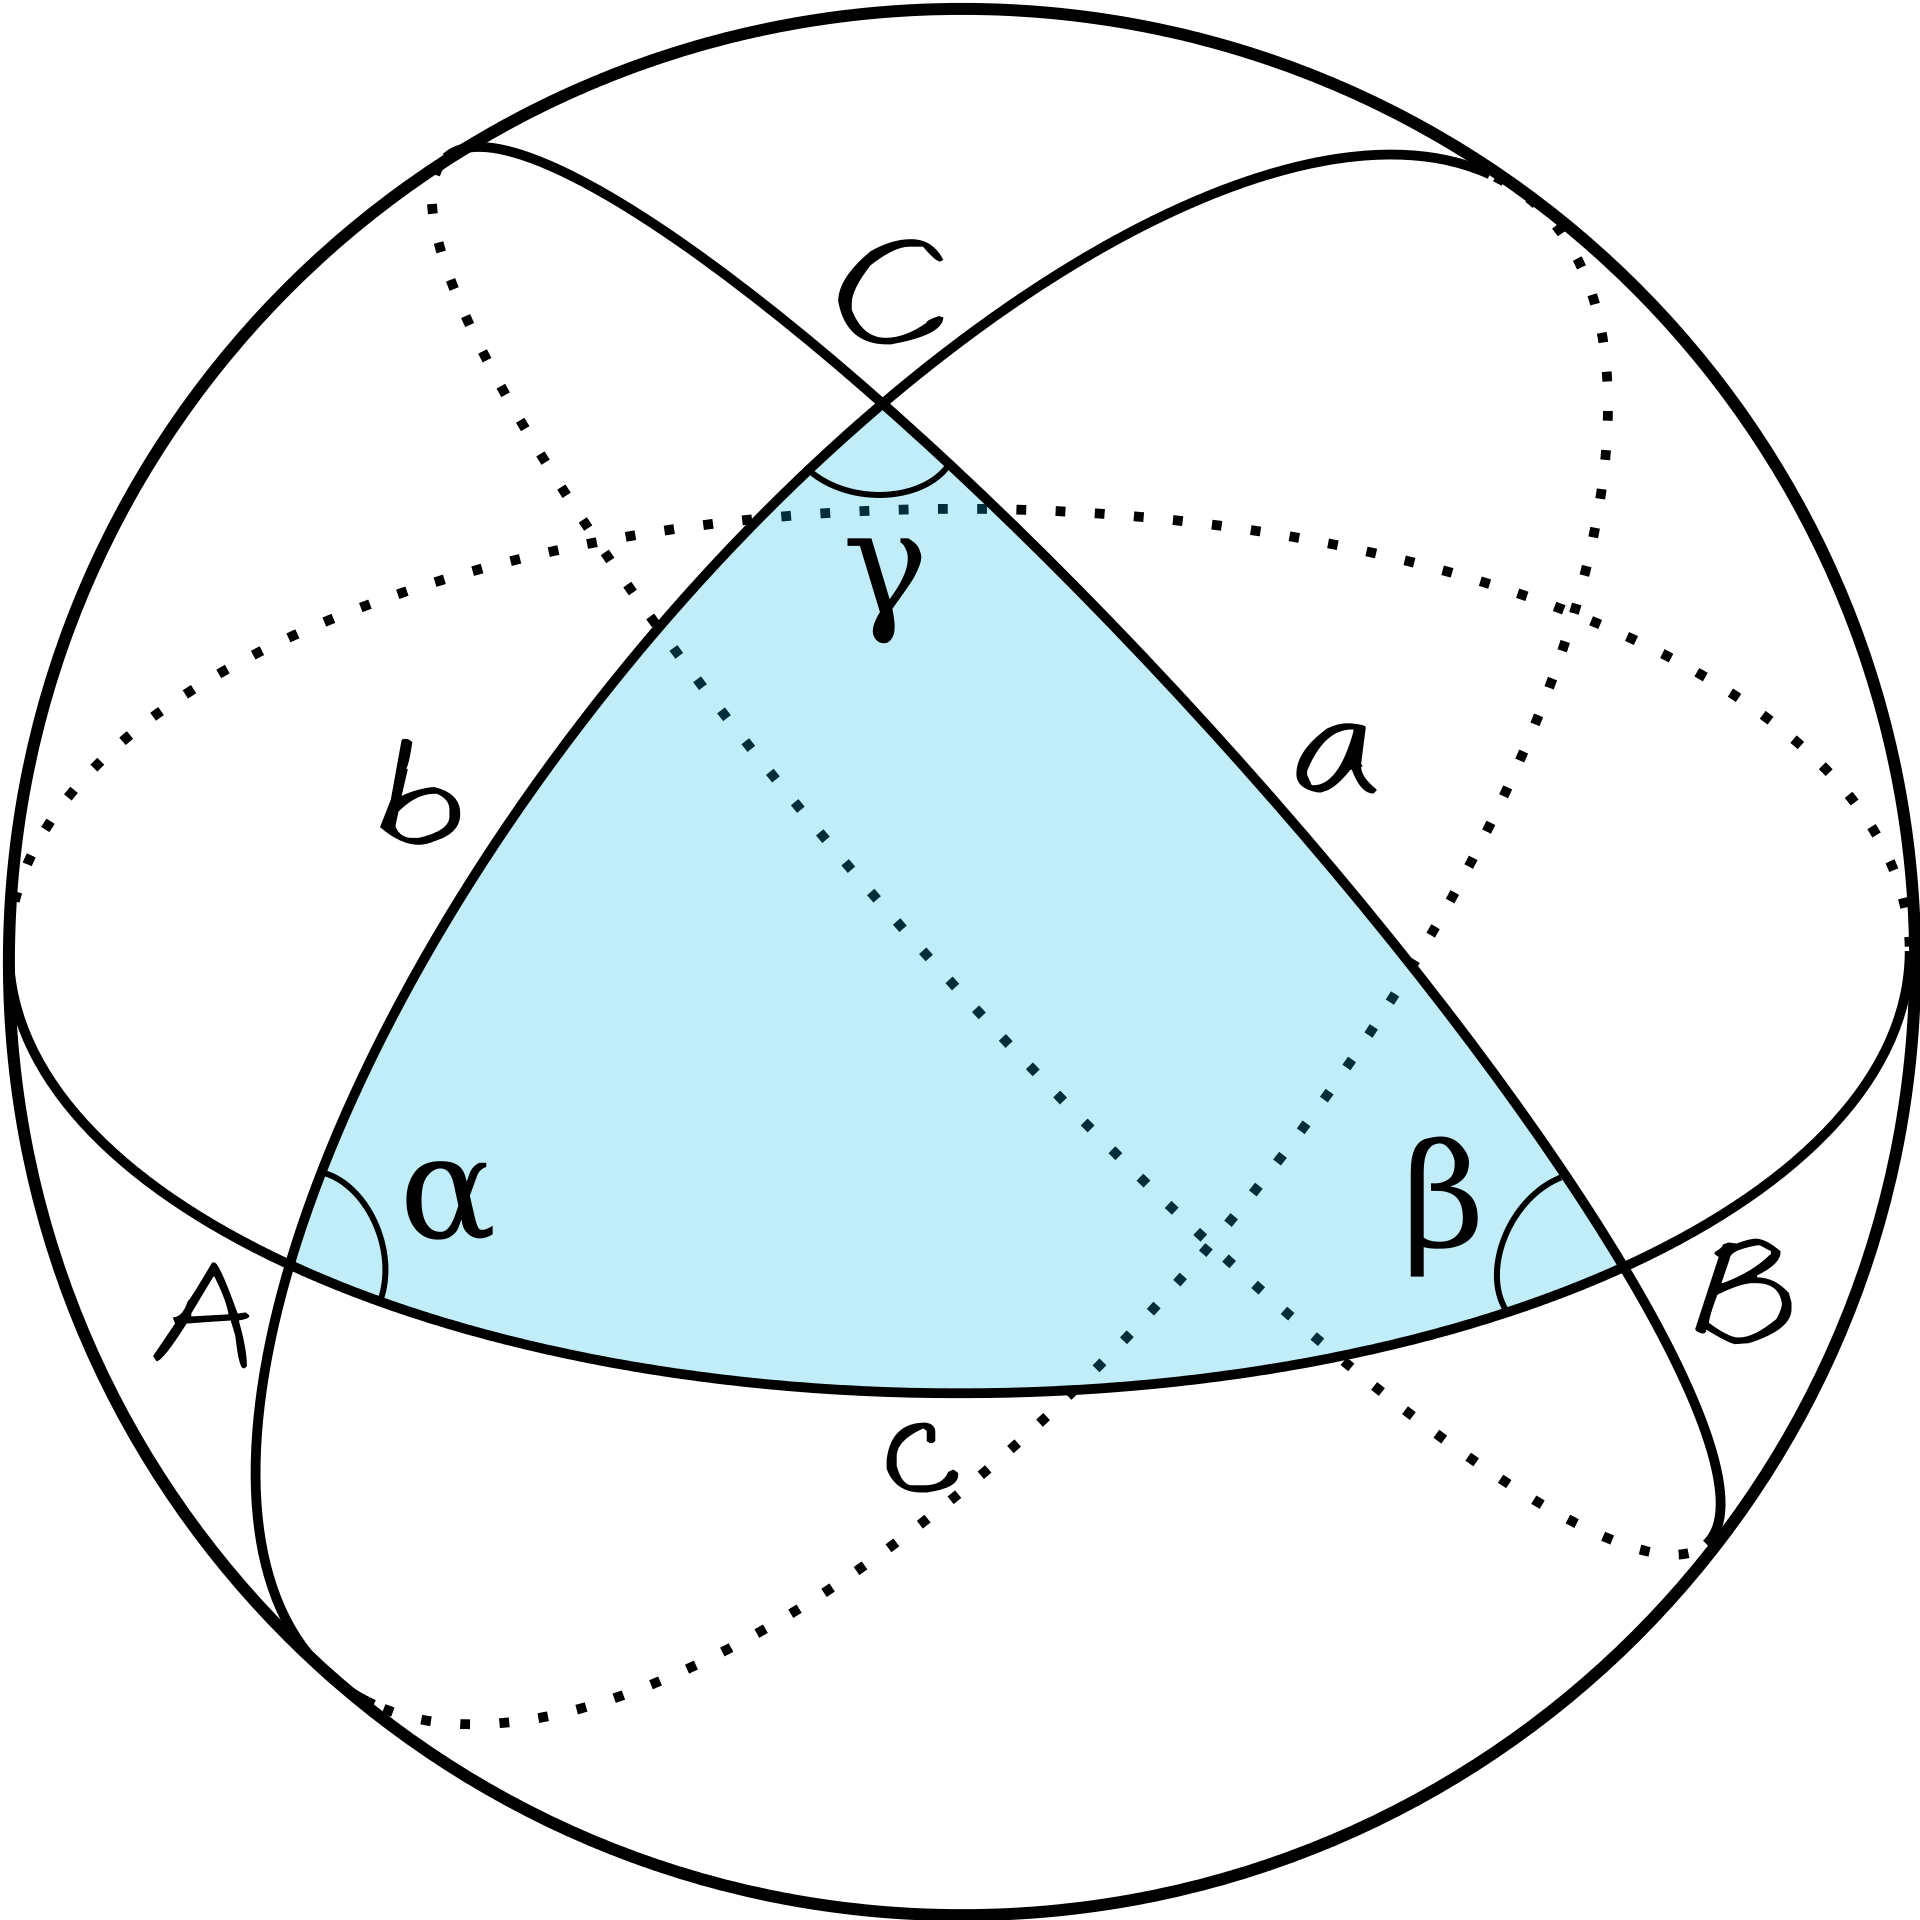
\includegraphics[width=0.3\textwidth]{sphere.png} & \hspace{0.5in} &
			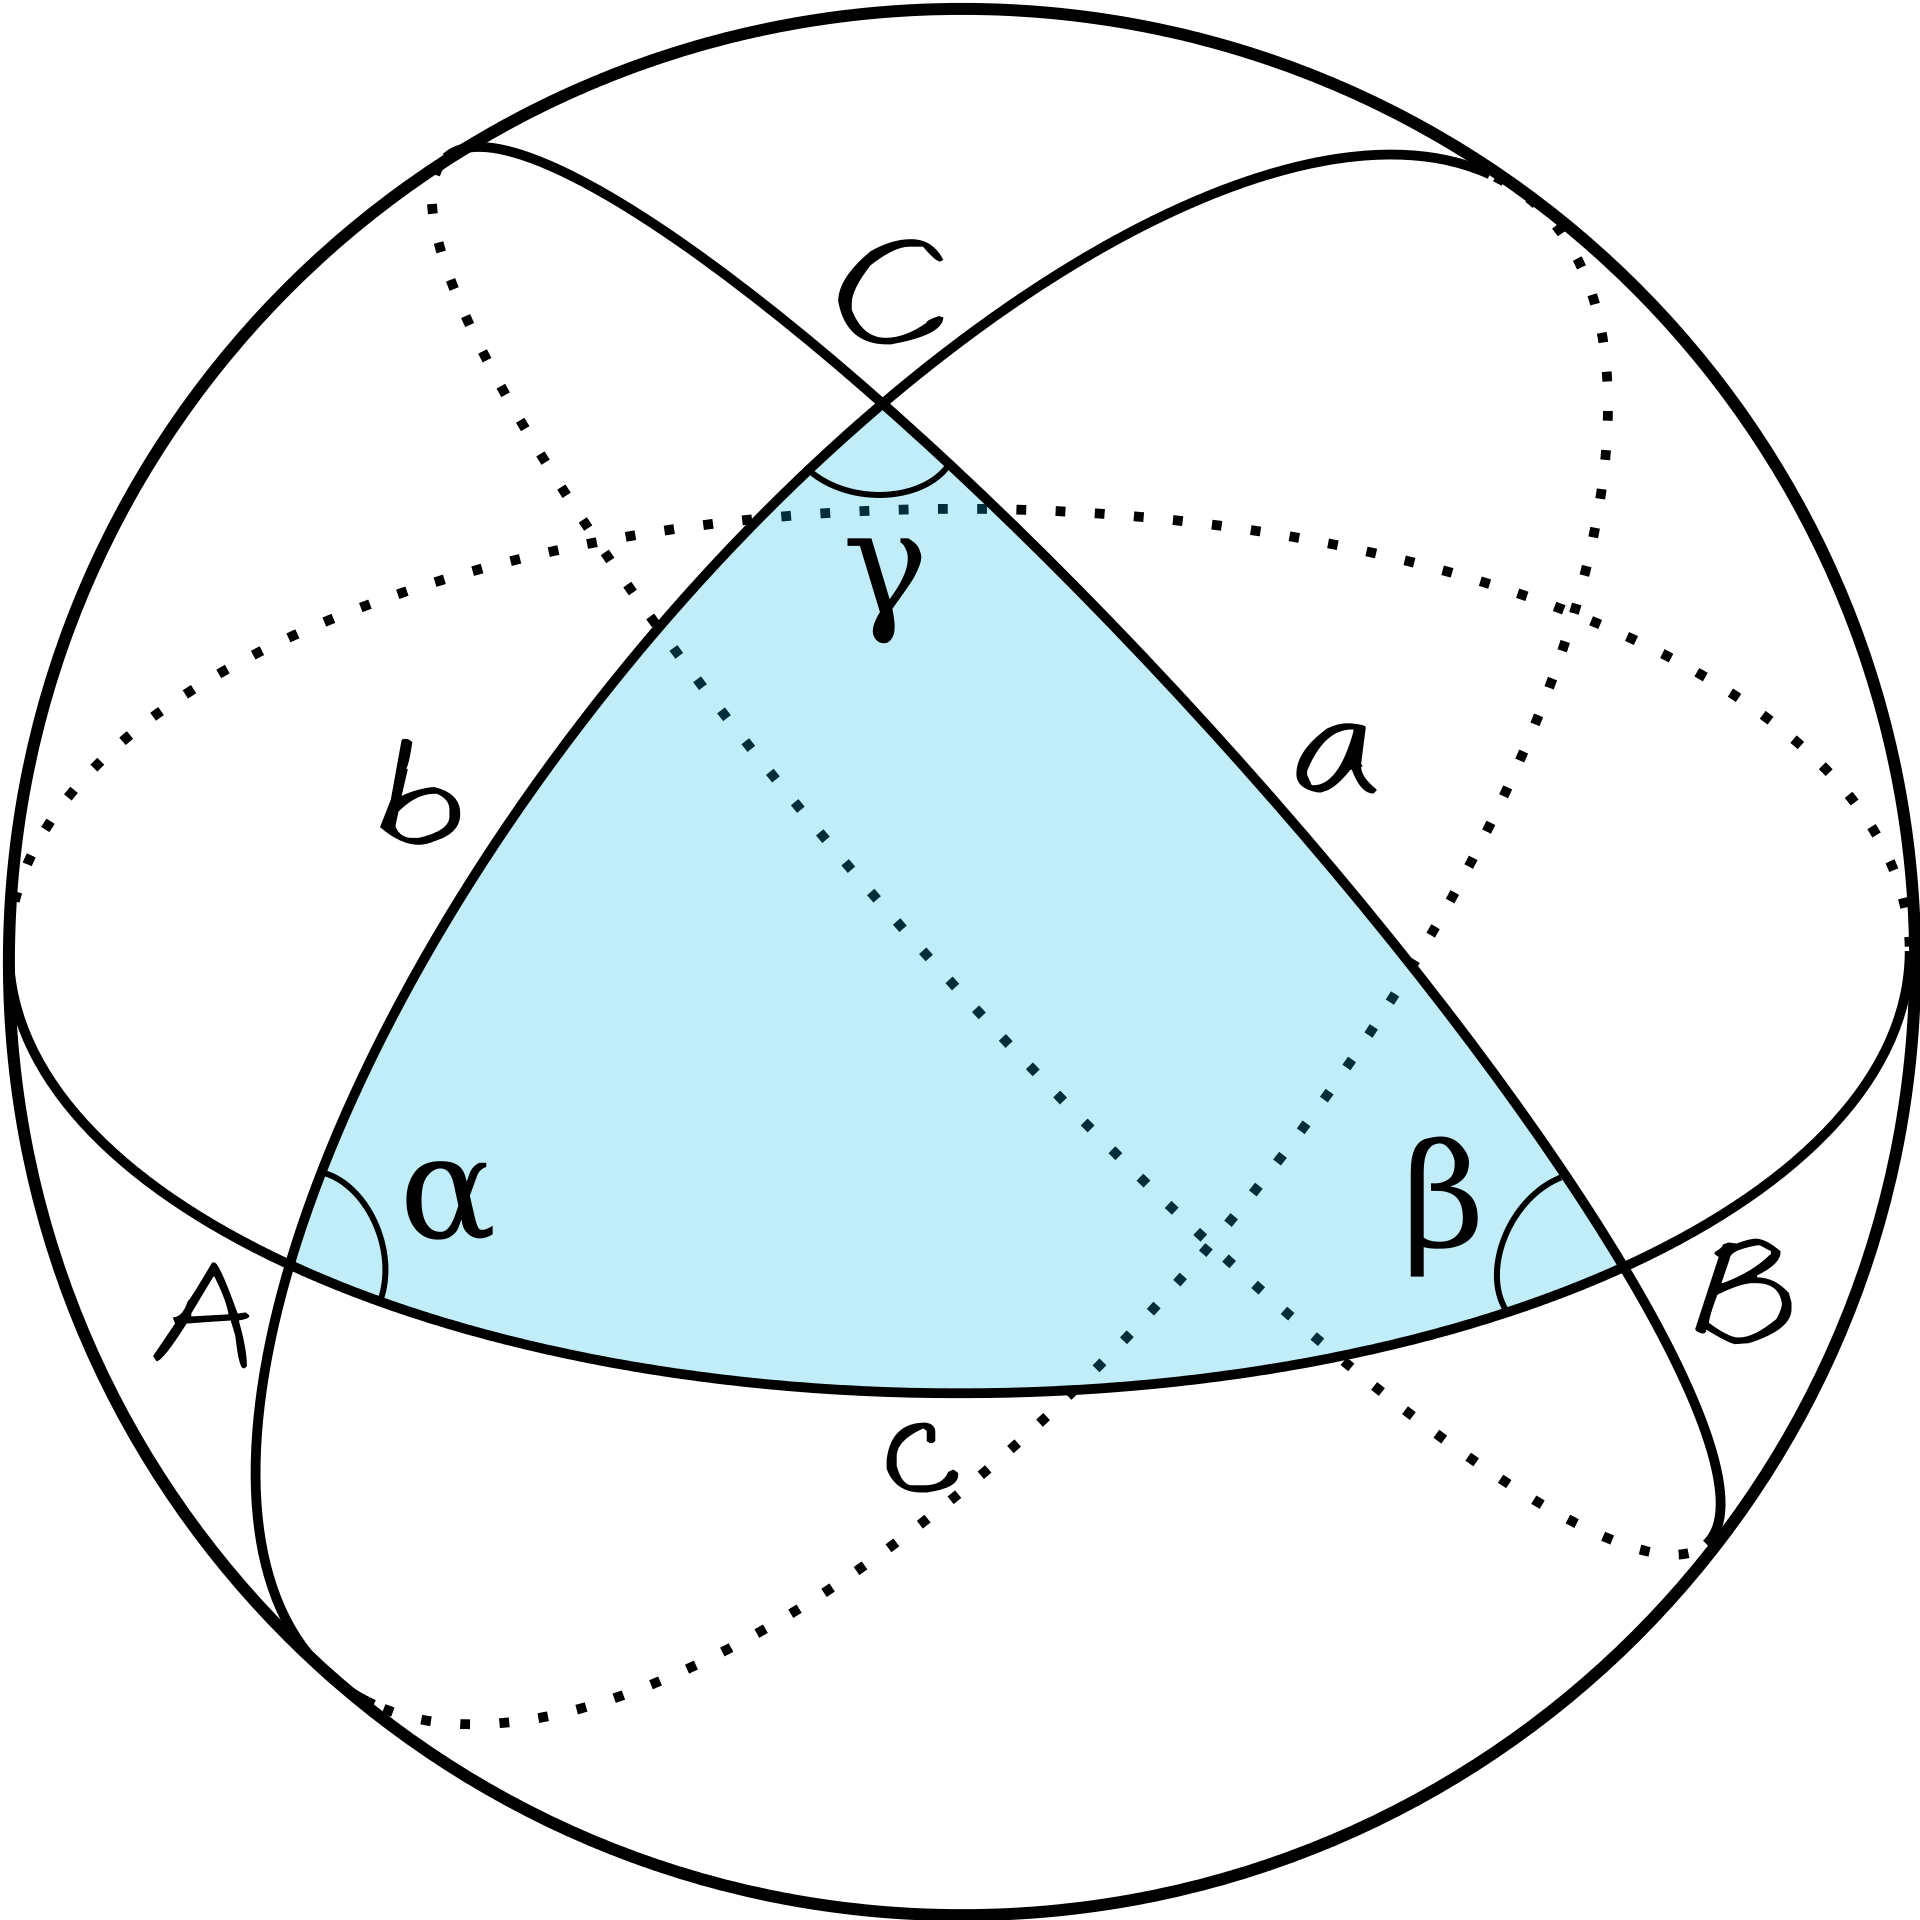
\includegraphics[width=0.3\textwidth]{sphere.png} \\
			(a) & & (b) \\[0.75in]
			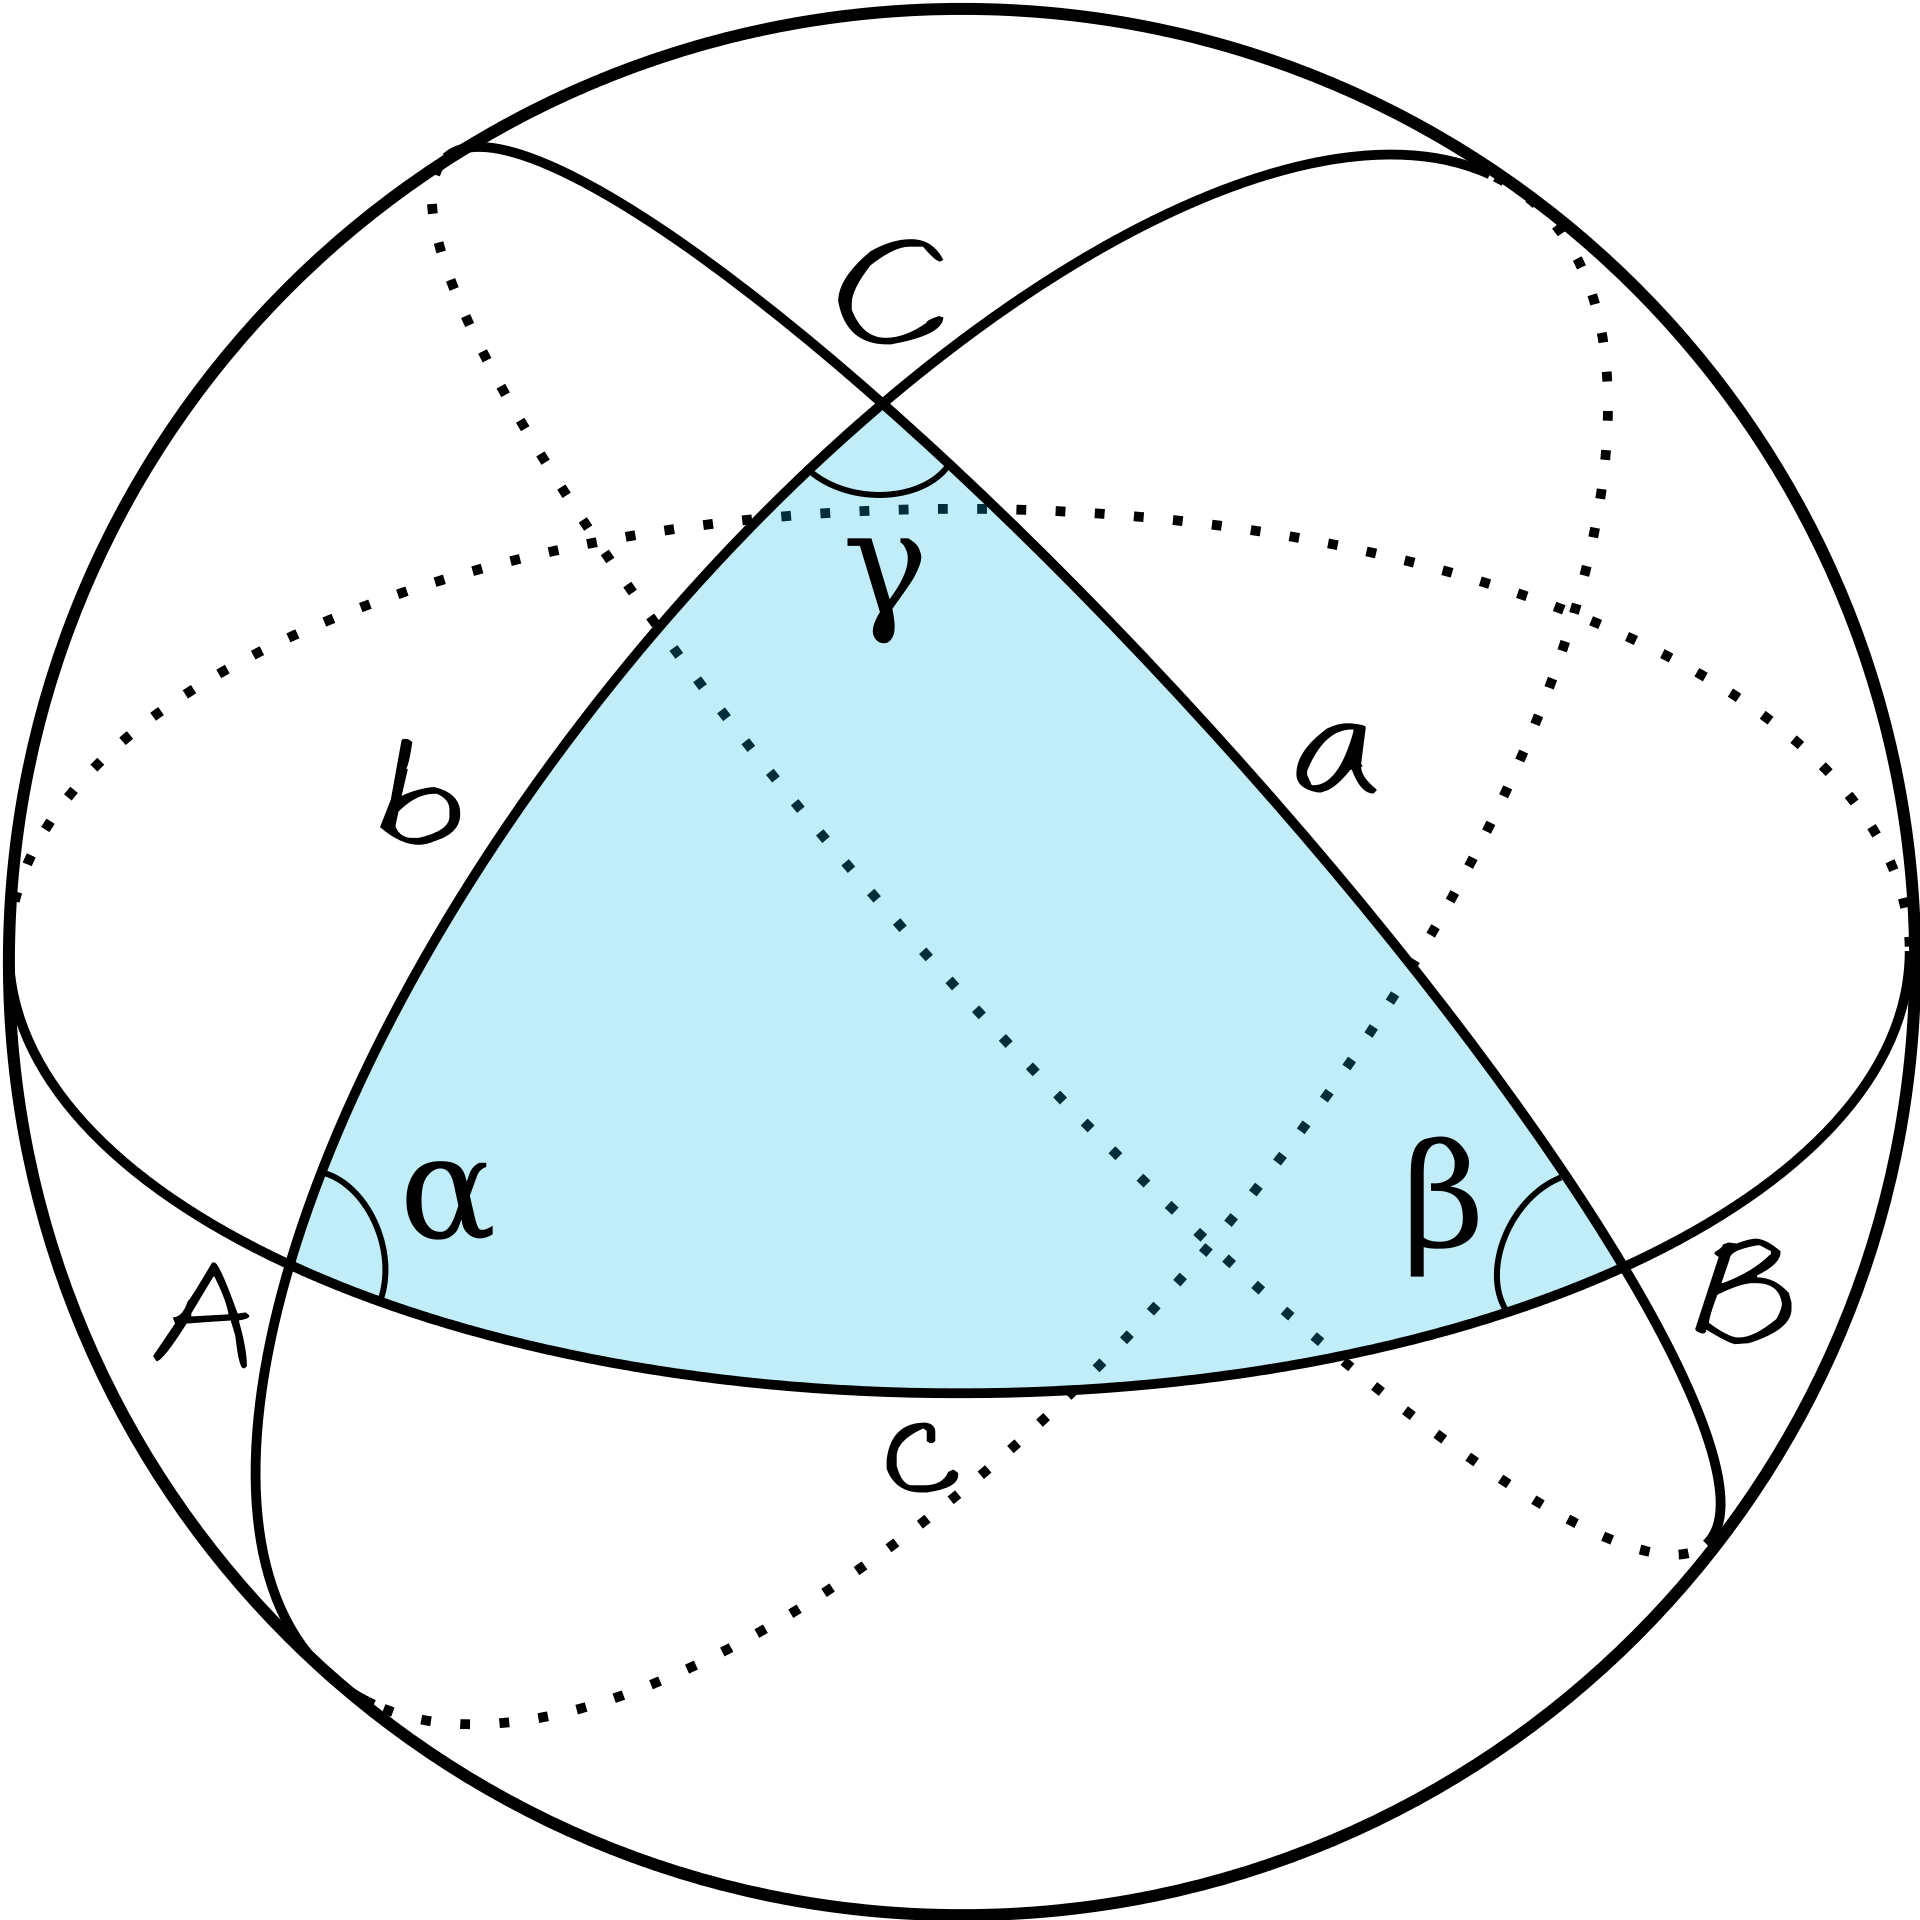
\includegraphics[width=0.3\textwidth]{sphere.png} & &
			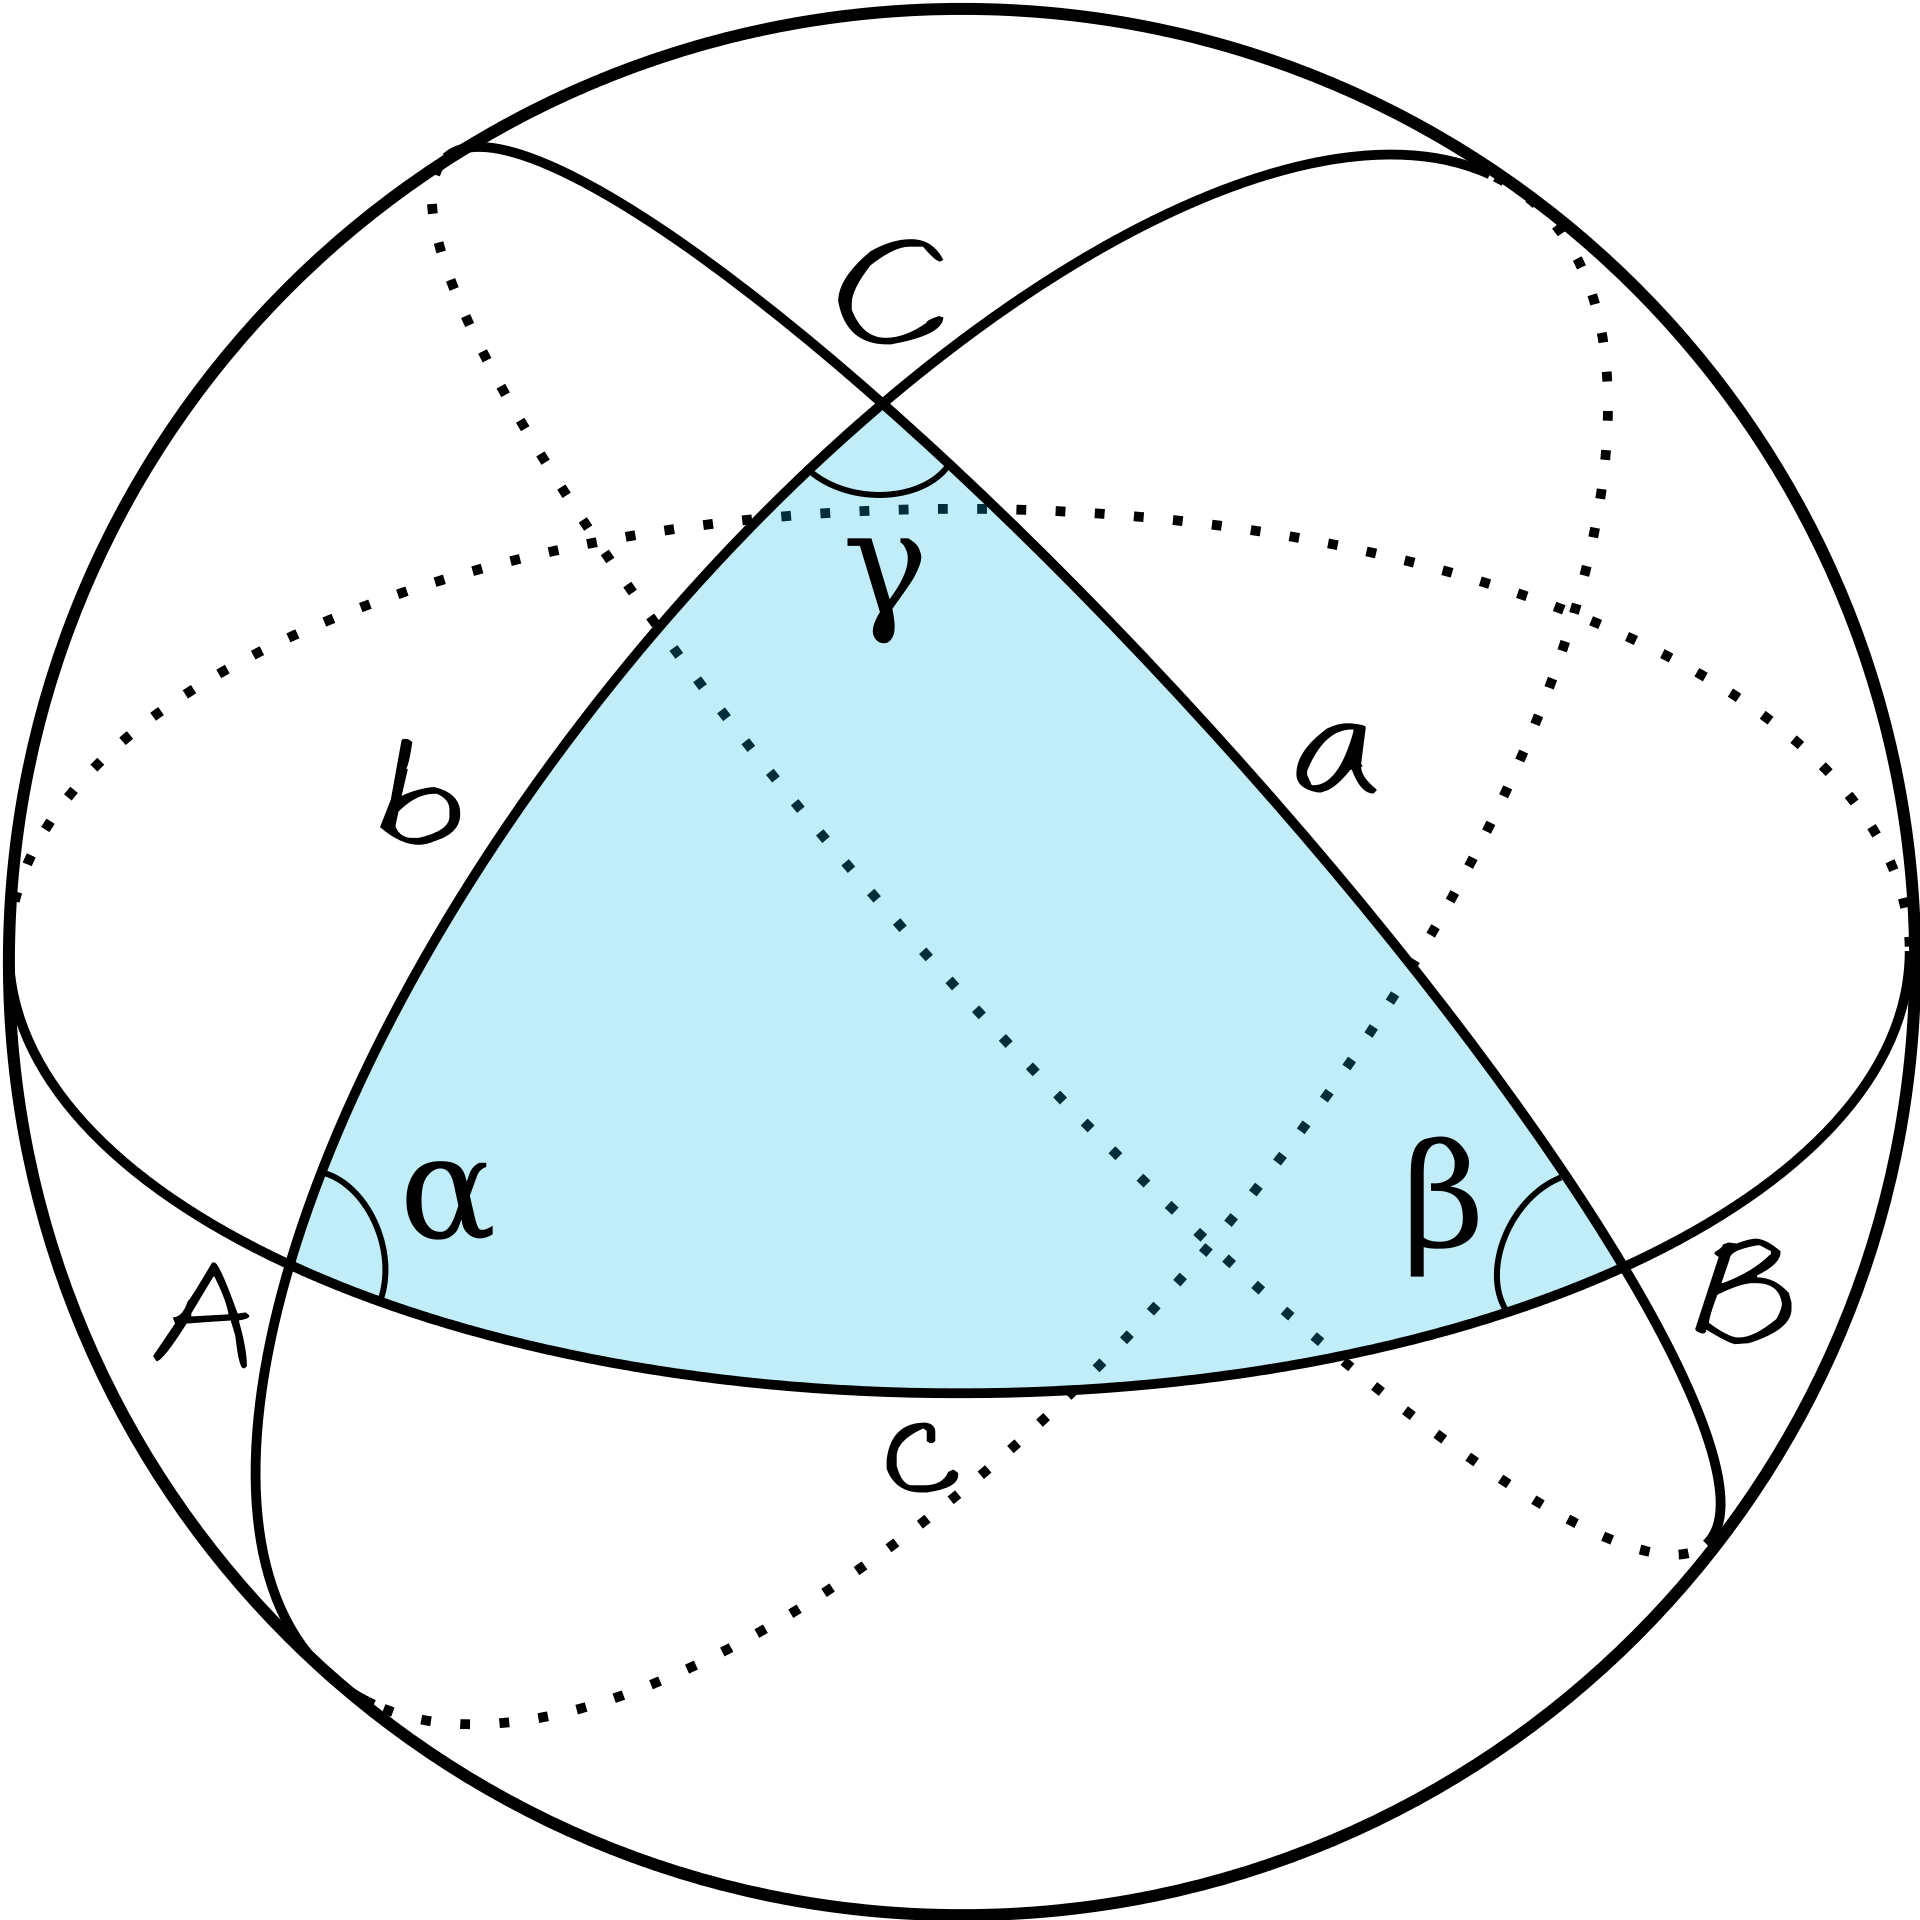
\includegraphics[width=0.3\textwidth]{sphere.png} \\
			(c) & & (d)
		\end{tabular}
		\caption{The areas (a) $2 \Asabg$, (b) $2 \Asa$, (c) $2 \Asb$, and (d) $2 \Asg$.}
		\label{f3d}
	\end{figure}
}